We simulated $w$ values at 10, 20, 30, 40 and 50.
Towards the bottom of \tty{viz.ipynb}, we have a small function that computes
the volume flow rate for a simulation as described above.
We use it to assemble the volume flows for these widths in both the 
periodic and non-periodic boundary conditions.
Here are the requested plots:

\begin{figure}[H]
    \centering
    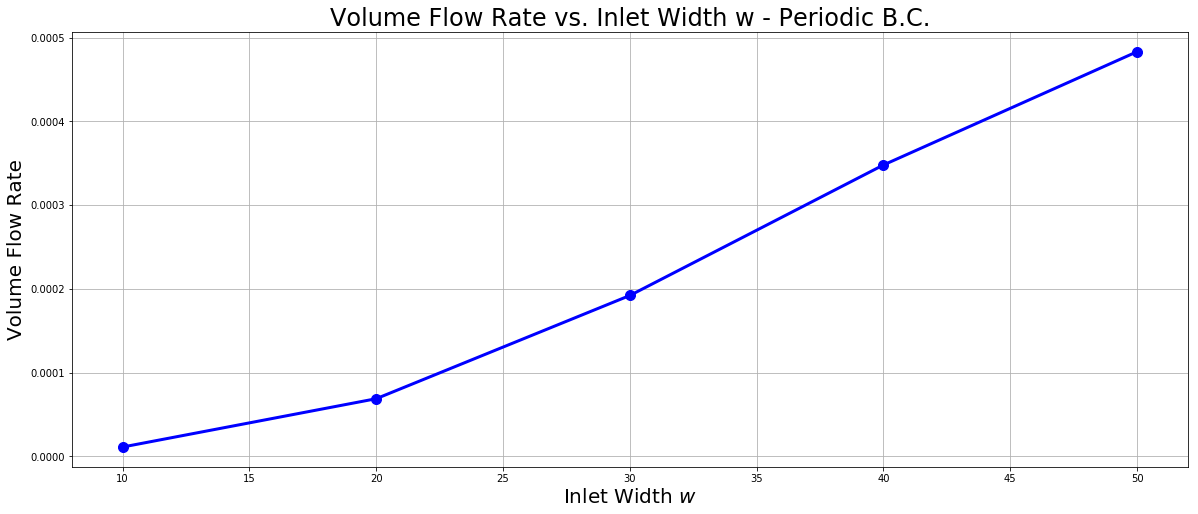
\includegraphics[width=0.85\textwidth]{lbm_pbc_flow_vs_w.png}
    \caption{Flow vs. Channel Width $w$ of the periodic channel.}
\end{figure}

\begin{figure}[H]
    \centering
    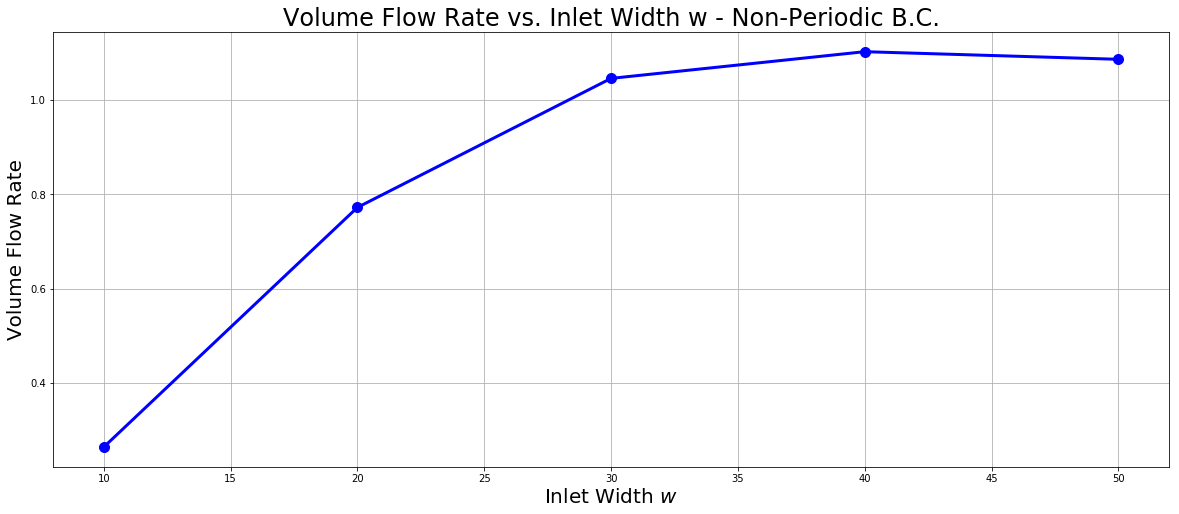
\includegraphics[width=0.85\textwidth]{lbm_mbc_flow_vs_w.png}
    \caption{Flow vs. Channel Width $w$ of the non-periodic channel.}
\end{figure}

As expected, we see that the volume flow rate increases for the periodic case with a roughly parabolic shape. The flow rate also increases for the non-periodic case, but plateaus past a width of 30. However, we need to be very careful with our intuition here, because we've standardized on a Reynolds number of 0.01 rather than a pressure gradient. Our intuition about how the flow depends on the width of the opening is based on varying the width while holding the pressure gradient constant. This simulation isn't calibrated that way, so it's measuring something slightly different, especially in the non-periodic case.